\section{Checking the candidate sets}
\label{app:probe}

Table~\ref{tab:probe} gives the audio probe for every candidate set. The probe
is a logistic regression on eight statistics of each standardised envelope that
do not change when the signal is rescaled: kurtosis, skew, Gini sparsity, the
range between the 5th and 95th percentiles, the fraction of near-silent samples,
and three frequency-band ratios. It is trained and tested on different audio
content, and picks the candidate it rates most likely to be attended. A candidate
set that does not give the answer away must score $1/K$.

\begin{table}[h]
\caption{\textbf{Audio-only acceptance probe}: what a linear reader takes from
the candidates alone, with no access to any recording. A shortcut-free
construction must sit at chance.}
\label{tab:probe}
\centering\small
\begin{tabular}{@{}llrrr@{}}
\toprule
Construction & & $K$ & Probe & Excess over chance \\
\midrule
Competing talkers                    & \cUnm{}      & 4 & \R{probe/raw/K4}        & \R{probe/raw/K4/excess} \\
\quad + distribution matching        & \cMat{}   & 4 & \R{probe/qmatch/K4}     & \R{probe/qmatch/K4/excess} \\
Same-talker temporal negatives       & \cSame{}    & 3 & \R{probe/shifted/K3}    & \R{probe/shifted/K3/excess} \\
\quad + distribution matching        & \cSameM{} & 3 & \R{probe/shifted_qm/K3} & \R{probe/shifted_qm/K3/excess} \\
Same-talker temporal negatives       & \cSame{}    & 2 & \R{probe/shifted/K2}    & \R{probe/shifted/K2/excess} \\
\quad + distribution matching        & \cSameM{} & 2 & \R{probe/shifted_qm/K2} & \R{probe/shifted_qm/K2/excess} \\
\bottomrule
\end{tabular}
\end{table}

\section{Encoder design}
\label{app:encoder}

Each stream goes through five dilated temporal convolutions
\citep{yu2016dilated} with dilations $1,2,4,8,16$ and GroupNorm
\citep{wu2018groupnorm} after each layer. The EEG first passes through a
$1{\times}1$ convolution that maps the electrodes to $8$ virtual sensors. Three
choices matter. \textbf{The window matches the brain response.} The encoder sees
$63$ samples ($0.98$\,s), about the time over which the cortical response to
speech unfolds \citep{lalor2009}. A much larger window would make the deepest
layers mostly see padding, which is the same in every window, so their output
would stop depending on the input. \textbf{There is no activation on the last
layer.} A rectified output has no negative values, so the cosine between any two
embeddings is squeezed into $[0,1]$, and the correlations the score depends on
would all sit close to one. \textbf{Padding is symmetric.} The brain responds to a
sound $100$ to $300$\,ms after it, so an encoder that looks only backward in time
cannot see the response. One-sided versions are used on purpose to restrict the
model to delays after, or before, the sound (Section~\ref{sec:res-mm}).

\section{Further limitations}
\label{app:limits}

\paragraph{Part of the four-way contribution can come from the trial.}
The attended talker is the same in every window of a trial, so a decoder that
recognises \emph{which trial} it is looking at already knows part of the answer.
The same-talker results do not have this issue, because all candidates there come
from the same trial and the same voice.

\paragraph{One room, sixteen listeners, no tuning.}
The data come from one room, one language and sixteen listeners, and the frozen
video stream in particular reads \emph{this} room. We did not tune any setting.
The numbers are therefore not tuned in our favour, but we also cannot claim they
are the best this model can reach.

\paragraph{The cause of the audio mark is not tested directly.}
Every recording is used in only one role, so the role and the recording cannot be
separated. The dataset's authors explain the mark by clipping during the loudness
adjustment \citep{maestro2026}, but the released data cannot test this directly.
No result depends on it: the probe measures how readable the mark is, whatever
its cause, and both fixes work either way. A dataset in which each recording is
the attended talker in some trials and an ignored one in others would remove the
mark at the source.

\section{Per-stream credit, drawn}
\label{app:creditfig}

\begin{figure}[h]
\centering
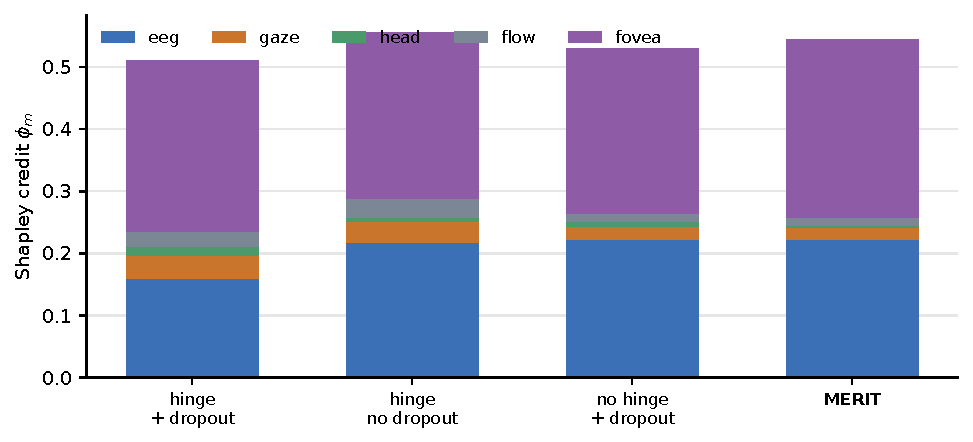
\includegraphics[width=0.72\textwidth]{figs/credit_bars.pdf}
\caption{\textbf{Shapley credit per stream}, stacked, for the four fused rows
of Table~\ref{tab:hinge}. Each bar's total height is that model's contribution
$v(M)-v(\emptyset)$, decomposed exactly. The question the figure answers is not
how tall the bars are but how much of each one is blue.}
\label{fig:credit}
\end{figure}

\section{Why this dataset, and not another}
\label{app:corpora}

Table~\ref{tab:corpora} compares the public AAD datasets we know of on the two
things that matter here: which streams are recorded next to the EEG, and whether
the listener is free to produce them.

\begin{table}[h]
\caption{\textbf{Public AAD corpora.} ``EOG'' denotes a few electro-oculography
electrodes recorded for artifact rejection, which is not calibrated gaze and
carries no head or scene information. The last column is the one that decides
whether modality freeloading is observable at all.}
\label{tab:corpora}
\centering\small
\resizebox{\textwidth}{!}{%
\begin{tabular}{@{}llllll@{}}
\toprule
Corpus & Gaze & Head & Scene video & Presentation & Listener \\
\midrule
DTU \citep{fuglsang2018dtu}        & 6 EOG & --- & --- & simulated rooms, earphones & soundproof booth \\
Four-speaker \citep{yan2024fourspeaker} & --- & --- & --- & 4 loudspeakers, anechoic & head fixed by chinrest \\
AV-GC-AAD \citep{geirnaert2024avgc} & 4 EOG & --- & --- & earphones, simulated HRTFs & gaze controlled by design \\
\textbf{MAESTRO} \citep{maestro2026} & \textbf{eye tracker} & \textbf{IMU} & \textbf{egocentric} & \textbf{6 loudspeakers, real room} & \textbf{unconstrained} \\
\bottomrule
\end{tabular}}
\end{table}

This pattern is not a flaw in those datasets. It is good design for the question
each one was built to answer. Holding the head and eyes still removes a source of
confusion, and AV-GC-AAD goes further and controls gaze on purpose, so that a
decoder that reads gaze can be caught. That makes it the best available test of
\emph{whether} a decoder uses gaze instead of the brain. But that is a yes-or-no
question about one stream. Our question is about amounts: when a listener
produces five streams at once, how does a fused decoder divide its evidence among
them, and how much stays with the brain? A dataset in which four of the five
streams are held fixed cannot answer it, because the effect has been designed
out. Testing \merit{} there would not be a harder test; it would be a test in
which the effect cannot appear.

Two parts of \merit{} do not need these streams and work on any matching
dataset: the audio probe, which only looks at the candidates, and the coupling
score, whose guarantee is a matter of arithmetic. We test both on two public
datasets in Appendices~\ref{app:external} and~\ref{app:externalcoupling}.

\section{The audio probe on two other datasets}
\label{app:external}

A check that only flags problems in the authors' own dataset is not yet a
reliable tool. We therefore ran the probe of Section~\ref{sec:failures}(i),
unchanged, on two public two-talker datasets collected by other groups:
KU~Leuven \citep{biesmans2017kul,das2019kuldata} and DTU \citep{fuglsang2018dtu},
with $16$ and $18$ listeners. Neither
records gaze, head motion or video, so only the audio part of \merit{} applies ---
which is the point, since the probe depends only on the candidates. We use one
envelope method for all three (power-law compression with exponent $0.6$, a
$20$\,Hz low-pass filter, and resampling to $64$\,Hz), standardise each
candidate, put the candidates in random order, and hold out whole stimulus pairs
for testing. Chance is $0.5$.

\begin{table}[h]
\caption{\textbf{The probe transfers, and it is calibrated.} Audio-only
two-way accuracy on $10$\,s windows, content-disjoint folds, no EEG. The last
column is the corpus's prior on which talker is attended; the probe tracks it.}
\label{tab:external}
\centering\small
\begin{tabular}{@{}lrrrrr@{}}
\toprule
Corpus & Listeners & Windows & Probe & Excess & Attended-role prior \\
\midrule
KU~Leuven & \R{extprobe/kul/w10/nlisteners} & \R{extprobe/kul/w10/nwin} & \textbf{\R{extprobe/kul/w10/probe}} & \textbf{\R{extprobe/kul/w10/excess}} & \R{extprior/kul/prior} \R{extprior/kul/role} \\
DTU & \R{extprobe/dtu/w10/nlisteners} & \R{extprobe/dtu/w10/nwin} & \R{extprobe/dtu/w10/probe} & \R{extprobe/dtu/w10/excess} & \R{extprior/dtu/prior} \R{extprior/dtu/role} \\
\bottomrule
\end{tabular}
\end{table}

\begin{table}[h]
\caption{\textbf{The same probe at four decision windows}, excess over chance.
On DTU, where the attended-role prior is balanced, no cell exceeds $0.005$. The
KU~Leuven excess is present at every window; its $30$\,s cell rests on
\R{extprobe/kul/w30/nwin} windows drawn from eight stimulus pairs and is the least
powered of the four.}
\label{tab:externalsweep}
\centering\small
\begin{tabular}{@{}lrrrr@{}}
\toprule
Corpus & $2$\,s & $5$\,s & $10$\,s & $30$\,s \\
\midrule
KU~Leuven, as released & \R{extprobe/kul/w2/excess} & \R{extprobe/kul/w5/excess} & \textbf{\R{extprobe/kul/w10/excess}} & \R{extprobe/kul/w30/excess} \\
\;\;distribution-matched & \R{extprobe/kul/w2/qmexcess} & \R{extprobe/kul/w5/qmexcess} & \R{extprobe/kul/w10/qmexcess} & \R{extprobe/kul/w30/qmexcess} \\
DTU, as released & \R{extprobe/dtu/w2/excess} & \R{extprobe/dtu/w5/excess} & \R{extprobe/dtu/w10/excess} & \R{extprobe/dtu/w30/excess} \\
\bottomrule
\end{tabular}
\end{table}

\paragraph{One dataset is clean, and that is what gives the other its meaning.}
Across four window lengths (Table~\ref{tab:externalsweep}) the probe stays within
$0.005$ of chance on DTU. The probe is not a warning that goes off everywhere.
Given two talkers who are attended about equally often, a classifier on eight
scale-free statistics cannot tell which one was attended, as it should not be
able to.

\paragraph{On KU~Leuven, the audio alone gives \R{extprobe/kul/w10/excess} above chance.}
On the most widely used AAD benchmark, the same classifier finds the attended
story with accuracy \R{extprobe/kul/w10/probe} on $10$\,s windows, against a
chance of $0.5$, and it is above chance at every window we tried. The cause is
not the audio mark of Section~\ref{sec:failures}(i) but an imbalance in the
labels: track~1 is the attended one in \R{extprior/kul/nrole} of
\R{extprior/kul/ntrials} trials, because the third part of the experiment repeats
the first, and in the first the listener always attends track~1. With two fixed
talkers and one of them attended far more often, the talker's identity
predicts the label, and voice identity is exactly what these statistics carry.
The dataset's own notes warn about two other problems, trial-level overfitting
and gaze; this is a third, separate one. No choice of split can remove it, because
it is part of the design, not of the split.

\paragraph{Matching the distributions only halves it.}
Quantile matching lowers the excess from \R{extprobe/kul/w10/excess} to
\R{extprobe/kul/w10/qmexcess}, and no further. This tells us something. Matching
makes every candidate's set of values the same, which removes the shape
statistics. It keeps each candidate's order in time, so the balance between
frequency bands survives, and with two fixed talkers that balance still reveals
who is speaking. When the problem is a label imbalance between two voices, the
fix is to balance the labels, not to match the distributions. This is a limit of
the candidate set we recommend, found by running our own tool on someone else's
data --- and it is why we report the probe for each dataset instead of calling
one candidate set safe everywhere.

\section{The coupling branch on two other datasets}
\label{app:externalcoupling}

The probe of Appendix~\ref{app:external} needs no model. Here we run the other
part of \merit{} that needs no behavioural stream --- the EEG coupling branch,
its shuffled baseline and the direction-in-time check --- on the same two
datasets. It runs through exactly the same code as every MAESTRO result: the
dataset is handed to the runner through the same data interface, and nothing
after that is changed. Candidates are matched, $K=2$, chance is $0.5$, and
$W=10$\,s. \emph{Same talker} replaces the competing talker with the attended
talker's own speech from another part of the same trial, so neither the talker's
identity nor their position can tell the candidates apart.

\begin{table}[h]
\caption{\textbf{What the full battery says about two public datasets.}
Accuracy and contribution for the unconstrained coupling branch, then
contribution with the branch confined to the causal ($+125\dots+1109$\,ms) and
mirrored acausal ($-1109\dots-125$\,ms) lag bands. \emph{Folds+} is for the
unconstrained branch. The last row is MAESTRO's same-talker $K=2$ result, the
reference for what a directional response looks like.}
\label{tab:externalcoupling}
\centering\small
\resizebox{\textwidth}{!}{%
\begin{tabular}{@{}lrrrrl@{}}
\toprule
& Accuracy & Contribution & Causal & Acausal & Folds+ \\
\midrule
KU~Leuven, within, competing & \R{extkulwithin/eeg_centred/within/acc} & \R{extkulwithin/eeg_centred/within/contrib} & \R{extkulwithin/eeg_causal/within/contrib} & \R{extkulwithin/eeg_acausal/within/contrib} & \R{extkulwithin/eeg_centred/within/pos} \\
KU~Leuven, within, same talker & \R{extkulwithinst/eeg_centred/within/acc} & \R{extkulwithinst/eeg_centred/within/contrib} & \R{extkulwithinst/eeg_causal/within/contrib} & \R{extkulwithinst/eeg_acausal/within/contrib} & \R{extkulwithinst/eeg_centred/within/pos} \\
KU~Leuven, LOSO, competing & \R{extkulloso/eeg_centred/loso/acc} & \R{extkulloso/eeg_centred/loso/contrib} & \R{extkulloso/eeg_causal/loso/contrib} & \R{extkulloso/eeg_acausal/loso/contrib} & \R{extkulloso/eeg_centred/loso/pos} \\
\midrule
DTU, within, competing & \R{extdtuwithin/eeg_centred/within/acc} & \R{extdtuwithin/eeg_centred/within/contrib} & \R{extdtuwithin/eeg_causal/within/contrib} & \R{extdtuwithin/eeg_acausal/within/contrib} & \R{extdtuwithin/eeg_centred/within/pos} \\
DTU, within, same talker & \R{extdtuwithinst/eeg_centred/within/acc} & \R{extdtuwithinst/eeg_centred/within/contrib} & \R{extdtuwithinst/eeg_causal/within/contrib} & \R{extdtuwithinst/eeg_acausal/within/contrib} & \R{extdtuwithinst/eeg_centred/within/pos} \\
DTU, LOSO, competing & \R{extdtuloso/eeg_centred/loso/acc} & \R{extdtuloso/eeg_centred/loso/contrib} & \R{extdtuloso/eeg_causal/loso/contrib} & \R{extdtuloso/eeg_acausal/loso/contrib} & \R{extdtuloso/eeg_centred/loso/pos} \\
\midrule
\midrule
\emph{MAESTRO, within, same talker} & \R{lag_mm/centred/within/acc} & \R{lag_mm/centred/within/contrib} & \textbf{\R{lag_mm/causal/within/contrib}} & \textbf{\R{lag_mm/acausal/within/contrib}} & \R{lag_mm/centred/within/pos} \\
\bottomrule
\end{tabular}}
\end{table}

\paragraph{The coupling branch transfers, and passes the hardest test we have.}
On KU~Leuven and DTU the coupling branch reaches
\R{extkulwithin/eeg_centred/within/acc} and \R{extdtuwithin/eeg_centred/within/acc}
within listeners, positive in every fold, and holds up on unseen listeners
(\R{extkulloso/eeg_centred/loso/acc} and \R{extdtuloso/eeg_centred/loso/acc},
positive in \R{extkulloso/eeg_centred/loso/pos} and
\R{extdtuloso/eeg_centred/loso/pos} folds). The same-talker test is the one that
matters. It removes talker identity, and with it a route that needs no timing at
all: the EEG could reveal \emph{which side} was attended --- through brain
activity that leans to one side, or through small eye movements, which are known
to affect datasets of this kind \citep{rotaru2024} --- and the audio could reveal
which talker is which. Accuracy does not fall under this test; it rises, to
\R{extkulwithinst/eeg_centred/within/acc} and \R{extdtuwithinst/eeg_centred/within/acc}.
Whatever the branch reads, it reads it from the timing.

\paragraph{But the direction-in-time check does not confirm it is the brain.}
On MAESTRO, limiting the coupling to delays after the sound gives about twice the
contribution of the mirror image before the sound
(\R{lag_mm/causal/within/contrib} against \R{lag_mm/acausal/within/contrib}), as a
response to the sound must. On KU~Leuven and DTU the two are the same in every row
of Table~\ref{tab:externalcoupling}. A match that depends on timing but not on its
direction is what a signal at \emph{zero} delay would give, spread equally into
both directions by the slow changes of the speech envelope itself. Both datasets
play the audio through in-ear phones close to the electrodes, and an electrical
leak of the sound into the recording is the classic zero-delay artifact; MAESTRO
plays it through loudspeakers across a room, and there the check passes. We think
this is the most likely explanation, but we have not shown it, and we do not count
the KU~Leuven or DTU accuracies as brain decoding.

\paragraph{Against published results, at the same window.}
Accuracy on these two datasets depends strongly on how the data are split.
\citet{alavi2026neurotoken} re-ran five recent decoders on KU~Leuven at $5$\,s,
once with each paper's own split and once with a split that holds out whole
trials, allows no overlap between training and test windows, and fits all
preprocessing on training trials only. Table~\ref{tab:published} gives the result
next to NeuroToken's own numbers and ours, all at $5$\,s. Chance is $0.5$.

\begin{table}[h]
\caption{\textbf{Two-talker accuracy at $5$\,s: with each paper's own split, and
without leakage.} The first five rows decode the \emph{direction} of attention
from EEG alone, and are NeuroToken's re-runs on KU~Leuven listeners $1$--$4$
\citep{alavi2026neurotoken}; the headline numbers in those papers are higher
still, $95$--$97\%$ at $1$\,s. NeuroToken and \merit{} decode the attended
\emph{talker} from EEG and the candidate speech. NeuroToken holds out whole trials;
\merit{} holds out whole stimuli and uses matched candidates. ``Unseen'' means
listeners not seen in training.}
\label{tab:published}
\centering\small
\begin{tabular}{@{}llrrr@{}}
\toprule
& & \multicolumn{2}{c}{KU~Leuven} & DTU \\
\cmidrule(lr){3-4}\cmidrule(lr){5-5}
Method & Decodes & own split & no leakage & no leakage \\
\midrule
DARNet \citep{yan2024darnet}         & direction & $0.895$ & $0.552$ & --- \\
ListenNet \citep{fan2025listennet}   & direction & $0.930$ & $0.484$ & --- \\
DBPNet \citep{ni2024dbpnet}          & direction & $0.884$ & $0.483$ & --- \\
DenseNet-3D \citep{xu2024densenet}   & direction & $0.864$ & $0.698$ & --- \\
SWIM \citep{zhang2025swim}           & direction & $0.644$ & $0.353$ & --- \\
\midrule
NeuroToken, within listeners         & talker & --- & $0.864$ & $0.837$ \\
NeuroToken, unseen listeners         & talker & --- & $0.634$ & $0.592$ \\
\midrule
\merit{}, within listeners           & talker & --- & \R{extkulwithin5/eeg_centred/within/acc} & \R{extdtuwithin5/eeg_centred/within/acc} \\
\merit{}, unseen listeners           & talker & --- & \R{extkulloso5/eeg_centred/loso/acc} & \R{extdtuloso5/eeg_centred/loso/acc} \\
\bottomrule
\end{tabular}
\end{table}

\paragraph{Reading the table.}
With each paper's own split, the direction decoders reach $0.64$ to $0.93$. Once
leakage is removed they fall by $17$ to $45$ points, to between $0.35$ and $0.70$,
and several land near or below chance: the published numbers mostly measured the
split, not the decoder. NeuroToken is the strongest prior result that survives a
split without leakage. \textbf{On unseen listeners, \merit{} is more accurate than
NeuroToken on both datasets}: \R{extkulloso5/eeg_centred/loso/acc} on
KU~Leuven and \R{extdtuloso5/eeg_centred/loso/acc} on DTU
(Table~\ref{tab:published}), and positive for every one of the
\R{extkulloso5/eeg_centred/loso/nfolds} and \R{extdtuloso5/eeg_centred/loso/nfolds}
held-out listeners. Within listeners it is not: NeuroToken is more accurate than
our \R{extkulwithin5/eeg_centred/within/acc} and
\R{extdtuwithin5/eeg_centred/within/acc} on both, and DenseNet-3D is also higher
on the four KU~Leuven listeners it was run on. The five direction decoders were re-run within
listeners only, so they have no unseen-listener number to compare. Two differences from our setting remain. First, NeuroToken holds
out whole trials, while we hold out whole stimuli. KU~Leuven repeats stories across
trials --- its third part replays the first --- so a split by trial can still put
the same story in training and test, and a split by stimulus cannot. Second, our
candidates are matched, while on KU~Leuven the candidates as released let the audio
alone reach \R{extprobe/kul/w5/excess} above chance at $5$\,s
(Table~\ref{tab:externalsweep}). For our own rows, the caution of this section still
applies: on these two datasets the direction-in-time check does not confirm that
the coupling branch reads a brain response. We have not run that check on the
other methods.

\paragraph{This is the argument of the paper, on other people's data.}
A standard evaluation would report $0.82$ on DTU and stop there. The audio probe
clears the candidates; the same-talker test rules out identity and position; and
the direction check then declines to confirm what is left. Each step is cheap, and
without the last one the number would have been reported as brain decoding.

\section{The hinge experiment on unseen listeners}
\label{app:hinge2loso}

\begin{table}[h]
\caption{\textbf{The $2\times2$ of Table~\ref{tab:hinge}, both protocols.}
$\phi_{\text{EEG}}$ is the EEG's Shapley credit; \emph{Folds+} counts
leave-one-listener-out folds with a positive contribution. No arm is best in
every column.}
\label{tab:hinge2loso}
\centering\small
\begin{tabular}{@{}lrrrrl@{}}
\toprule
& \multicolumn{2}{c}{Within-subject} & \multicolumn{3}{c}{Leave-one-listener-out} \\
\cmidrule(lr){2-3}\cmidrule(lr){4-6}
Arm & Accuracy & $\phi_{\text{EEG}}$ & Accuracy & $\phi_{\text{EEG}}$ & Folds+ \\
\midrule
Hinge, modality dropout & \R{v2hinge2/H1_hinge_drop/within/acc} & \R{v2hinge2/H1_hinge_drop/within/shap/eeg} & \R{v2hinge2loso/H1_hinge_drop/loso/acc} & \R{v2hinge2loso/H1_hinge_drop/loso/shap/eeg} & \R{v2hinge2loso/H1_hinge_drop/loso/pos} \\
No hinge, modality dropout & \R{v2hinge2/H2_nohinge_drop/within/acc} & \R{v2hinge2/H2_nohinge_drop/within/shap/eeg} & \R{v2hinge2loso/H2_nohinge_drop/loso/acc} & \R{v2hinge2loso/H2_nohinge_drop/loso/shap/eeg} & \R{v2hinge2loso/H2_nohinge_drop/loso/pos} \\
\textbf{\merit{}} (no hinge, no dropout) & \R{v2hinge2/H4_nohinge_nodrop/within/acc} & \R{v2hinge2/H4_nohinge_nodrop/within/shap/eeg} & \R{v2hinge2loso/H4_nohinge_nodrop/loso/acc} & \R{v2hinge2loso/H4_nohinge_nodrop/loso/shap/eeg} & \R{v2hinge2loso/H4_nohinge_nodrop/loso/pos} \\
Hinge, no dropout & \R{v2hinge2/H3_hinge_nodrop/within/acc} & \R{v2hinge2/H3_hinge_nodrop/within/shap/eeg} & \R{v2hinge2loso/H3_hinge_nodrop/loso/acc} & \R{v2hinge2loso/H3_hinge_nodrop/loso/shap/eeg} & \R{v2hinge2loso/H3_hinge_nodrop/loso/pos} \\
\bottomrule
\end{tabular}
\end{table}

The order of the four models changes between the two splits. The model with the
hinge and no dropout is the most accurate within listeners and the least accurate
on unseen ones. In both pairs, the model without the hinge keeps more credit on
the brain on unseen listeners. \merit{} is the model without the hinge and
without dropout: it has the most EEG credit on unseen listeners and ties for the
most within listeners.

\section{Every stream set, both splits}
\label{app:loso}

Table~\ref{tab:streams} gives every stream set within listeners, and
Table~\ref{tab:streamsloso} gives the same models on unseen listeners. Both use
per-window decisions at $W=10$\,s.

\begin{table}[t]
\caption{\textbf{Accuracy, null and contribution by stream set}, within-subject
(five content-disjoint folds), \cMat{}, $W=10$\,s, chance $0.25$.
\emph{Folds+} counts folds with a positive contribution. The
leave-one-listener-out counterpart is Table~\ref{tab:streamsloso}.}
\label{tab:streams}
\centering\small
\begin{tabular}{@{}lrrrrl@{}}
\toprule
Streams & Accuracy & Null & Contribution & $p$ & Folds+ \\
\midrule
EEG & \R{streams/eeg/within/acc} & \R{streams/eeg/within/null} & \R{streams/eeg/within/contrib} & \R{streams/eeg/within/p} & \R{streams/eeg/within/pos} \\
EEG + gaze & \R{streams/eeg_gaze/within/acc} & \R{streams/eeg_gaze/within/null} & \R{streams/eeg_gaze/within/contrib} & \R{streams/eeg_gaze/within/p} & \R{streams/eeg_gaze/within/pos} \\
EEG + head & \R{streams/eeg_imu/within/acc} & \R{streams/eeg_imu/within/null} & \R{streams/eeg_imu/within/contrib} & \R{streams/eeg_imu/within/p} & \R{streams/eeg_imu/within/pos} \\
EEG + flow & \R{streams/eeg_flow/within/acc} & \R{streams/eeg_flow/within/null} & \R{streams/eeg_flow/within/contrib} & \R{streams/eeg_flow/within/p} & \R{streams/eeg_flow/within/pos} \\
EEG + fovea & \R{streams/eeg_fovea/within/acc} & \R{streams/eeg_fovea/within/null} & \R{streams/eeg_fovea/within/contrib} & \R{streams/eeg_fovea/within/p} & \R{streams/eeg_fovea/within/pos} \\
Behaviour only & \R{streams/behaviour/within/acc} & \R{streams/behaviour/within/null} & \R{streams/behaviour/within/contrib} & \R{streams/behaviour/within/p} & \R{streams/behaviour/within/pos} \\
\textbf{All five} & \R{streams/all/within/acc} & \R{streams/all/within/null} & \R{streams/all/within/contrib} & \R{streams/all/within/p} & \R{streams/all/within/pos} \\
\bottomrule
\end{tabular}
\end{table}

\begin{table}[h]
\caption{\textbf{Leave-one-listener-out}, sixteen folds, each with a held-out
listener on held-out content. \cMat{}, $W=10$\,s, chance $0.25$.}
\label{tab:streamsloso}
\centering\small
\begin{tabular}{@{}lrrrrl@{}}
\toprule
Streams & Accuracy & Null & Contribution & $p$ & Folds+ \\
\midrule
EEG & \R{loso/eeg/loso/acc} & \R{loso/eeg/loso/null} & \R{loso/eeg/loso/contrib} & \R{loso/eeg/loso/p} & \R{loso/eeg/loso/pos} \\
EEG + gaze & \R{loso/eeg_gaze/loso/acc} & \R{loso/eeg_gaze/loso/null} & \R{loso/eeg_gaze/loso/contrib} & \R{loso/eeg_gaze/loso/p} & \R{loso/eeg_gaze/loso/pos} \\
EEG + head & \R{loso/eeg_imu/loso/acc} & \R{loso/eeg_imu/loso/null} & \R{loso/eeg_imu/loso/contrib} & \R{loso/eeg_imu/loso/p} & \R{loso/eeg_imu/loso/pos} \\
EEG + flow & \R{loso/eeg_flow/loso/acc} & \R{loso/eeg_flow/loso/null} & \R{loso/eeg_flow/loso/contrib} & \R{loso/eeg_flow/loso/p} & \R{loso/eeg_flow/loso/pos} \\
EEG + fovea & \R{loso/eeg_fovea/loso/acc} & \R{loso/eeg_fovea/loso/null} & \R{loso/eeg_fovea/loso/contrib} & \R{loso/eeg_fovea/loso/p} & \R{loso/eeg_fovea/loso/pos} \\
Behaviour only & \R{loso/behaviour/loso/acc} & \R{loso/behaviour/loso/null} & \R{loso/behaviour/loso/contrib} & \R{loso/behaviour/loso/p} & \R{loso/behaviour/loso/pos} \\
\textbf{All five} & \R{loso/all/loso/acc} & \R{loso/all/loso/null} & \R{loso/all/loso/contrib} & \R{loso/all/loso/p} & \R{loso/all/loso/pos} \\
\bottomrule
\end{tabular}
\end{table}

\section{Checks on the EEG signal}
\label{app:more}

Table~\ref{tab:mm} gives the same-talker results and the direction-in-time
check. Figure~\ref{fig:window} shows how the contribution changes with the
decision window.

\begin{table}[h]
\caption{\textbf{Orienting-free decoding and neural directionality.} EEG only
unless stated, within-subject, $W=10$\,s. Same-talker candidates are the attended
talker at different times, so slot index carries no spatial meaning and no
orienting cue can help. The lag band is set by the encoder's direction plus an
eight-sample shift; a contribution as large in the acausal band would indicate a
shared artifact rather than envelope tracking.}
\label{tab:mm}
\centering\small
\setlength{\tabcolsep}{5pt}
\begin{tabular}{@{}llllrrrr@{}}
\toprule
Candidates & $K$ & Streams & EEG visible at & Chance & Accuracy & Null & Contribution \\
\midrule
\cSameM{} & 3 & EEG      & centred & 0.333 & \R{mm3/eeg/within/acc} & \R{mm3/eeg/within/null} & \textbf{\R{mm3/eeg/within/contrib}}\\
\cSameM{} & 3 & all five & centred & 0.333 & \R{mm3/all/within/acc} & \R{mm3/all/within/null} & \textbf{\R{mm3/all/within/contrib}}\\
\cSameM{} & 2 & EEG      & centred & 0.500 & \R{mm2/eeg/within/acc} & \R{mm2/eeg/within/null} & \textbf{\R{mm2/eeg/within/contrib}}\\
\cSameM{} & 2 & all five & centred & 0.500 & \R{mm2/all/within/acc} & \R{mm2/all/within/null} & \textbf{\R{mm2/all/within/contrib}}\\
\midrule
\cMat{}   & 4 & EEG & $+125\dots+1109$\,ms & 0.250 & \R{lag_qm/causal/within/acc} & \R{lag_qm/causal/within/null} & \textbf{\R{lag_qm/causal/within/contrib}}\\
\cMat{}   & 4 & EEG & $-1109\dots-125$\,ms & 0.250 & \R{lag_qm/acausal/within/acc} & \R{lag_qm/acausal/within/null} & \textbf{\R{lag_qm/acausal/within/contrib}}\\
\cSameM{} & 2 & EEG & $+125\dots+1109$\,ms & 0.500 & \R{lag_mm/causal/within/acc} & \R{lag_mm/causal/within/null} & \textbf{\R{lag_mm/causal/within/contrib}}\\
\cSameM{} & 2 & EEG & $-1109\dots-125$\,ms & 0.500 & \R{lag_mm/acausal/within/acc} & \R{lag_mm/acausal/within/null} & \textbf{\R{lag_mm/acausal/within/contrib}}\\
\bottomrule
\end{tabular}
\end{table}

\begin{figure}[h]
\centering
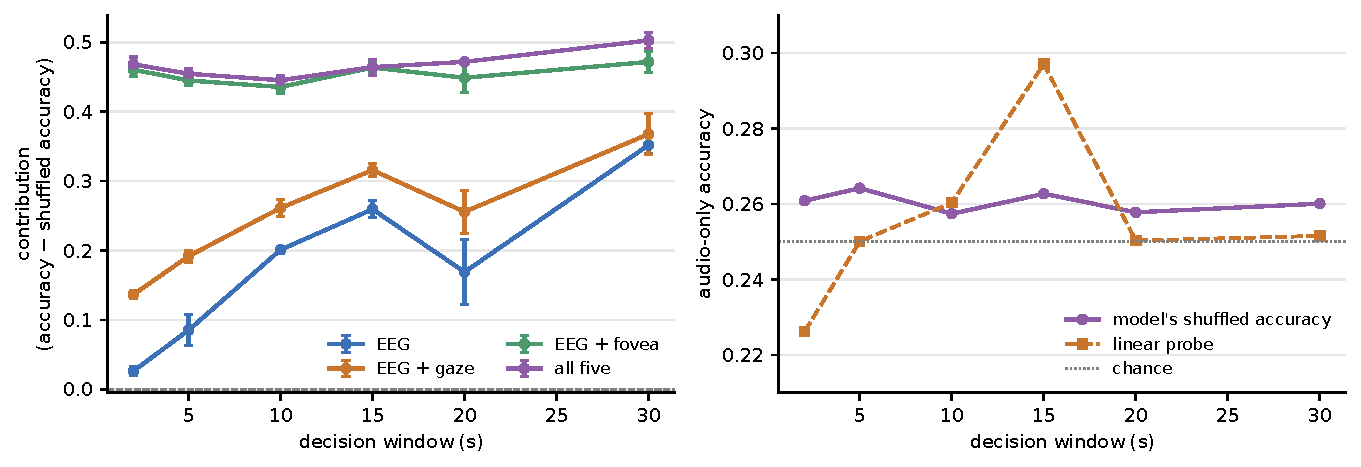
\includegraphics[width=0.86\textwidth]{figs/window_sweep.pdf}
\caption{\textbf{Contribution against decision-window length}, within-listener,
\cMat{}. Left: contribution for the four stream sets measured at every
window; the eleven stream sets at $2$ and $5$\,s are in Table~\ref{tab:shortwin}.
Right: the full model's shuffled accuracy, which is what the contribution
subtracts, and the linear audio probe, both measured at each window. The model's
shuffled accuracy stays within $0.015$ of chance throughout; the probe varies
more, between $0.23$ and $0.30$.}
\label{fig:window}
\end{figure}

\subsection{Short decision windows, by stream set}
\label{app:shortwin}

Figure~\ref{fig:window} changes the window for a few stream sets.
Table~\ref{tab:shortwin} does the opposite at the two shortest windows: every
stream set at $W=2$\,s and $W=5$\,s, within listeners, one decision per window,
with half-window hops. The rows extend Figure~\ref{fig:window} downward and can be
compared directly with a benchmark that decides one window at a time. Short
windows are where the problem this paper is about is strongest. The behavioural
streams show \emph{where} the listener faces, which a two-second look already
settles. The coupling branch needs time for a brain response to build up, and its
own window is already $0.98$\,s. The table shows this clearly. At $W=2$\,s the
EEG alone contributes \R{w2/eeg/within/contrib}, while the frozen foveal embedding
alone reaches \R{w2/fovea/within/acc} with a contribution of
\R{w2/fovea/within/contrib}, and the full five-stream model reaches
\R{w2/all/within/acc}. At that window a fused accuracy is almost entirely about
where the listener was looking. It should not be read as a brain result, and
without the per-stream split nothing in the headline number would say so.

\begin{table}[h]
\caption{\textbf{Every stream set at the two shortest decision windows},
within-subject (content-disjoint, five folds), \cMat{}, $K=4$, chance
$0.25$, hop $=W/2$. \emph{Contribution} is accuracy minus the model's own
permutation null; $p$ is the permutation $p$-value, floored at $0.048$ for twenty
permutations. The first block is single streams, the second EEG paired with each
behavioural stream.}
\label{tab:shortwin}
\centering\small
\resizebox{\textwidth}{!}{%
\begin{tabular}{@{}lrrrrrrrr@{}}
\toprule
& \multicolumn{4}{c}{$W=2$\,s} & \multicolumn{4}{c}{$W=5$\,s} \\
\cmidrule(lr){2-5}\cmidrule(lr){6-9}
Streams & Acc. & Null & Contrib. & $p$ & Acc. & Null & Contrib. & $p$ \\
\midrule
EEG & \R{w2/eeg/within/acc} & \R{w2/eeg/within/null} & \R{w2/eeg/within/contrib} & \R{w2/eeg/within/p} & \R{w5/eeg/within/acc} & \R{w5/eeg/within/null} & \R{w5/eeg/within/contrib} & \R{w5/eeg/within/p} \\
gaze & \R{w2/gaze/within/acc} & \R{w2/gaze/within/null} & \R{w2/gaze/within/contrib} & \R{w2/gaze/within/p} & \R{w5/gaze/within/acc} & \R{w5/gaze/within/null} & \R{w5/gaze/within/contrib} & \R{w5/gaze/within/p} \\
head motion & \R{w2/imu/within/acc} & \R{w2/imu/within/null} & \R{w2/imu/within/contrib} & \R{w2/imu/within/p} & \R{w5/imu/within/acc} & \R{w5/imu/within/null} & \R{w5/imu/within/contrib} & \R{w5/imu/within/p} \\
optical flow & \R{w2/flow/within/acc} & \R{w2/flow/within/null} & \R{w2/flow/within/contrib} & \R{w2/flow/within/p} & \R{w5/flow/within/acc} & \R{w5/flow/within/null} & \R{w5/flow/within/contrib} & \R{w5/flow/within/p} \\
fovea (V-JEPA\,2) & \R{w2/fovea/within/acc} & \R{w2/fovea/within/null} & \R{w2/fovea/within/contrib} & \R{w2/fovea/within/p} & \R{w5/fovea/within/acc} & \R{w5/fovea/within/null} & \R{w5/fovea/within/contrib} & \R{w5/fovea/within/p} \\
behaviour (all four) & \R{w2/behaviour/within/acc} & \R{w2/behaviour/within/null} & \R{w2/behaviour/within/contrib} & \R{w2/behaviour/within/p} & \R{w5/behaviour/within/acc} & \R{w5/behaviour/within/null} & \R{w5/behaviour/within/contrib} & \R{w5/behaviour/within/p} \\
\midrule
EEG + gaze & \R{w2/eeg_gaze/within/acc} & \R{w2/eeg_gaze/within/null} & \R{w2/eeg_gaze/within/contrib} & \R{w2/eeg_gaze/within/p} & \R{w5/eeg_gaze/within/acc} & \R{w5/eeg_gaze/within/null} & \R{w5/eeg_gaze/within/contrib} & \R{w5/eeg_gaze/within/p} \\
EEG + head & \R{w2/eeg_imu/within/acc} & \R{w2/eeg_imu/within/null} & \R{w2/eeg_imu/within/contrib} & \R{w2/eeg_imu/within/p} & \R{w5/eeg_imu/within/acc} & \R{w5/eeg_imu/within/null} & \R{w5/eeg_imu/within/contrib} & \R{w5/eeg_imu/within/p} \\
EEG + flow & \R{w2/eeg_flow/within/acc} & \R{w2/eeg_flow/within/null} & \R{w2/eeg_flow/within/contrib} & \R{w2/eeg_flow/within/p} & \R{w5/eeg_flow/within/acc} & \R{w5/eeg_flow/within/null} & \R{w5/eeg_flow/within/contrib} & \R{w5/eeg_flow/within/p} \\
EEG + fovea & \R{w2/eeg_fovea/within/acc} & \R{w2/eeg_fovea/within/null} & \R{w2/eeg_fovea/within/contrib} & \R{w2/eeg_fovea/within/p} & \R{w5/eeg_fovea/within/acc} & \R{w5/eeg_fovea/within/null} & \R{w5/eeg_fovea/within/contrib} & \R{w5/eeg_fovea/within/p} \\
\textbf{all five} & \R{w2/all/within/acc} & \R{w2/all/within/null} & \R{w2/all/within/contrib} & \R{w2/all/within/p} & \R{w5/all/within/acc} & \R{w5/all/within/null} & \R{w5/all/within/contrib} & \R{w5/all/within/p} \\
\bottomrule
\end{tabular}}
\end{table}

\section{The hinge experiment at ten seconds}
\label{app:hingew10}

Table~\ref{tab:hingew10} repeats the hinge experiment at the earlier setting
($W=10$\,s, one decision per window). It also changes how checkpoints are chosen,
which Table~\ref{tab:hinge} does not. Choosing by contribution instead of by
accuracy is the one training choice that raises the EEG's credit.

\begin{table}[h]
\caption{\textbf{Hinge, selection rule and modality dropout at $W=10$\,s}, per-window decisions --- the earlier operating point, kept because it varies the selection rule, which Table~\ref{tab:hinge} does not. Identical
streams, data and folds; within-subject, \cMat{}, $W=10$\,s, chance
$0.25$. $\phi_m$ is Shapley credit and sums to the contribution by construction.
The single-stream EEG model is shown for reference.}
\label{tab:hingew10}
\centering\small
\setlength{\tabcolsep}{4pt}
\begin{tabular}{@{}lrrrrrrrr@{}}
\toprule
& & & & \multicolumn{5}{c}{Shapley credit $\phi_m$}\\
\cmidrule(l){5-9}
Model & Accuracy & Null & Contrib. & EEG & gaze & head & flow & fovea \\
\midrule
EEG alone (reference)
 & \R{streams/eeg/within/acc} & \R{streams/eeg/within/null} & \R{streams/eeg/within/contrib}
 & \R{streams/eeg/within/contrib} & --- & --- & --- & --- \\
\midrule
No hinge, accuracy-selected
 & \R{hinge/all_nohinge_accsel/within/acc} & \R{hinge/all_nohinge_accsel/within/null} & \R{hinge/all_nohinge_accsel/within/contrib}
 & \R{hinge/all_nohinge_accsel/within/shap/eeg} & \R{hinge/all_nohinge_accsel/within/shap/gaze} & \R{hinge/all_nohinge_accsel/within/shap/imu} & \R{hinge/all_nohinge_accsel/within/shap/video} & \R{hinge/all_nohinge_accsel/within/shap/fovea} \\
No hinge, credit-selected
 & \R{hinge/all_nohinge_credsel/within/acc} & \R{hinge/all_nohinge_credsel/within/null} & \R{hinge/all_nohinge_credsel/within/contrib}
 & \R{hinge/all_nohinge_credsel/within/shap/eeg} & \R{hinge/all_nohinge_credsel/within/shap/gaze} & \R{hinge/all_nohinge_credsel/within/shap/imu} & \R{hinge/all_nohinge_credsel/within/shap/video} & \R{hinge/all_nohinge_credsel/within/shap/fovea} \\
Hinge, accuracy-selected
 & \R{hinge/all_hinge_accsel/within/acc} & \R{hinge/all_hinge_accsel/within/null} & \R{hinge/all_hinge_accsel/within/contrib}
 & \R{hinge/all_hinge_accsel/within/shap/eeg} & \R{hinge/all_hinge_accsel/within/shap/gaze} & \R{hinge/all_hinge_accsel/within/shap/imu} & \R{hinge/all_hinge_accsel/within/shap/video} & \R{hinge/all_hinge_accsel/within/shap/fovea} \\
Hinge, credit-selected
 & \R{hinge/all_hinge_credsel/within/acc} & \R{hinge/all_hinge_credsel/within/null} & \R{hinge/all_hinge_credsel/within/contrib}
 & \textbf{\R{hinge/all_hinge_credsel/within/shap/eeg}} & \R{hinge/all_hinge_credsel/within/shap/gaze} & \R{hinge/all_hinge_credsel/within/shap/imu} & \R{hinge/all_hinge_credsel/within/shap/video} & \R{hinge/all_hinge_credsel/within/shap/fovea} \\
\midrule
Hinge, uniform weights
 & \R{hinge/all_hinge_uniform/within/acc} & \R{hinge/all_hinge_uniform/within/null} & \R{hinge/all_hinge_uniform/within/contrib}
 & \R{hinge/all_hinge_uniform/within/shap/eeg} & \R{hinge/all_hinge_uniform/within/shap/gaze} & \R{hinge/all_hinge_uniform/within/shap/imu} & \R{hinge/all_hinge_uniform/within/shap/video} & \R{hinge/all_hinge_uniform/within/shap/fovea} \\
Hinge, no modality dropout
 & \R{hinge/all_hinge_nodrop/within/acc} & \R{hinge/all_hinge_nodrop/within/null} & \R{hinge/all_hinge_nodrop/within/contrib}
 & \R{hinge/all_hinge_nodrop/within/shap/eeg} & \R{hinge/all_hinge_nodrop/within/shap/gaze} & \R{hinge/all_hinge_nodrop/within/shap/imu} & \R{hinge/all_hinge_nodrop/within/shap/video} & \R{hinge/all_hinge_nodrop/within/shap/fovea} \\
No hinge, no modality dropout
 & \R{hinge/all_nohinge_nodrop/within/acc} & \R{hinge/all_nohinge_nodrop/within/null} & \R{hinge/all_nohinge_nodrop/within/contrib}
 & \R{hinge/all_nohinge_nodrop/within/shap/eeg} & \R{hinge/all_nohinge_nodrop/within/shap/gaze} & \R{hinge/all_nohinge_nodrop/within/shap/imu} & \R{hinge/all_nohinge_nodrop/within/shap/video} & \R{hinge/all_nohinge_nodrop/within/shap/fovea} \\
\bottomrule
\end{tabular}
\end{table}

\section{The training objective, explained}
\label{app:objective}

Equation~\ref{eq:loss} gives the loss. This section explains two choices behind
it. \textbf{Why the contrastive term uses one listener at a time.} Raw EEG
identifies the listener with accuracy $0.90$ in a sixteen-way test, against a
chance of $0.0625$. In a batch that mixes listeners, the contrastive term could
match EEG to speech by recognising the listener, which says nothing about
attention. Every batch is therefore drawn from a single listener. \textbf{Why the
contrastive term and the anti-collapse term cannot be satisfied by collapse.} If
the EEG encoder outputs a vector that does not change over time, the time-centred
score gives $s(e,a)=0$ for every pair, so every entry of $S$ in
$\mathcal{L}_{\text{con}}$ is zero and the loss is exactly $\log B$, its value at
chance. And the first part of $\mathcal{L}_{\text{col}}$ measures
exactly the spread over time that such an encoder has lost. \merit{} trains
without modality dropout; the dropout models of Table~\ref{tab:hinge} drop each
stream with probability $0.3$, never all of them at once, and fill a dropped
stream with zeros so the fusion layer always runs.

\section{Reproducibility}
\label{app:repro}

The decoder, the data code and all tests are one package with one configuration
file, and every experiment is one command. The main results come from:

\begin{quote}\small\ttfamily
\# Table 1 and Appendix \ref{app:hinge2loso}: the four fused models, both splits\\
python -m src.main data=merit model=merit runner=merit\_hinge2 \$CROP \textbackslash\\
\quad data.euclidean\_align=true data.audio\_feats=env\_onset\\
python -m src.main data=merit model=merit runner=merit\_hinge2loso0 \$CROP ...\\
\# Table 2: the EEG-only ladder\\
python -m src.main data=merit model=merit runner=merit\_ladder2 \$CROP \textbackslash\\
\quad data.audio\_feats=env\_onset\\
\# Appendices: stream sets, short windows, other datasets\\
python -m src.main data=merit model=merit runner=merit\_streams\\
python -m src.main data=merit model=merit runner=merit\_winmod0 data.window\_sec=2 data.hop\_sec=1\\
python -m src.main data=external model=merit runner=merit\_external data.corpus=dtu\\
python -m src.main mode=certify data=merit model=merit runner=merit
\end{quote}
where \texttt{\$CROP} is \texttt{data.window\_sec=30 data.hop\_sec=15
data.crop\_len=640 data.n\_train\_crops=8 data.n\_eval\_crops=5}. The job scripts
that ran each experiment are released with the code.

The models inside one run share one dataset and one set of folds, so a difference
between two rows comes from the models alone. At test time the order of the
candidates is fixed by each window's index, so every model sees exactly the same
inputs. Every number in the paper is written from the run outputs by a script and
inserted automatically, never typed by hand, and a result is only used once every
fold of its run has finished.

\section{Hyper-parameters}
\label{app:hp}

\begin{table}[h]
\centering\small
\caption{Settings. None were tuned; each was set once from first principles.}
\begin{tabular}{@{}ll@{}}
\toprule
Item & Value \\
\midrule
Sampling rate / window / hop            & $64$\,Hz / $10$\,s / $5$\,s for per-window results (sweep: $2,5,10,15,20,30$\,s at $50\%$ hop) \\
Per-trial decisions (\merit{})          & $10$\,s crops of $30$\,s trials: $8$ random crops per trial when training, $5$ fixed crops at test; window scores summed per trial \\
Stream channels                         & EEG $32$ ($64$ on KU~Leuven and DTU), gaze $6$, head $6$, flow $4$, fovea $1024$ (frozen) \\
Descriptor width $D$ / layers           & $16$ / $5$ (dilations $1,2,4,8,16$; RF $63$ samples $=0.98$\,s)\\
Spatial filters (EEG)                   & $8$\\
Normalisation / activation              & GroupNorm($4$ groups) after every conv; no activation on the last\\
Dropout / modality dropout              & $0.1$ / none in \merit{}; $0.3$ in the dropout models of Table~\ref{tab:hinge} (never all streams; dropped streams filled with zeros) \\
Delays (\merit{})                       & EEG encoder sees only delays after the sound, offset $8$ samples ($+125$ to $+1109$\,ms) \\
Listener correction (\merit{})          & rank-$2$ correction of the EEG channels per listener; in the fused model the EEG is also whitened per listener (not in the EEG-only ladder) \\
Audio channels (\merit{})               & envelope and its rectified derivative (speech onsets) \\
Coupling temperature                    & learned, initialised at $1/0.07$\\
Optimiser / lr / weight decay           & AdamW / $10^{-3}$ / $10^{-4}$; grad-norm clip $1.0$\\
Batch                                   & $32$, drawn from a single listener\\
Schedule                                & lr $\times0.5$ after $5$ epochs without improvement; $\le50$ epochs; patience $12$\\
Label smoothing                         & $0.1$\\
Loss weights (Eq.~\ref{eq:loss})       & task $1.0$ (label smoothing $0.1$); auxiliary $0.3$; contrastive $1.0$; EEG null hinge $0.5$ (margin $\mu=0.5$); anti-collapse $0.1$ ($\gamma=0.5$); adversary $0.3$ \\
Contribution hinge (Eq.~\ref{eq:hinge}) & none in \merit{}; weight $0.5$, margin $\delta=0.3$ in the hinge models \\
Hinge weights                           & Eq.~\ref{eq:gate} in Table~\ref{tab:hinge}; $\lambda_m=\mathrm{clip}((\kappa-c_m)/\kappa,0,1)$, $\kappa=0.05$, in Table~\ref{tab:hingew10} \\
Checkpoint choice                       & Eq.~\ref{eq:criterion}, $\beta=1$ (accuracy recorded as well) \\
Permutations                            & $3$ on inner validation; $20$ at test; $5$ draws per Shapley coalition\\
Splits                                  & within: $5$ content-disjoint folds, $20\%$ inner val (content-disjoint)\\
                                        & LOSO: $16$ folds, $20\%$ global content holdout, inner val listener-disjoint\\
\bottomrule
\end{tabular}
\end{table}

\section{Why the Shapley credits add up}
\label{app:additivity}

Equation~\ref{eq:shapley} guarantees $\sum_m\phi_m=v(M)-v(\emptyset)$ exactly.
The code reports both sides for every run as a check, and they agree to the
printed precision in every result in this paper. All $2^5=32$ subsets are
computed rather than sampled, and the same shuffles are reused across subsets, so
a difference between two subsets is not shuffle noise. The cost is mostly in
re-scoring, not re-encoding, because the stream embeddings and audio embeddings
are computed once per evaluation.

Two cautions. First, $\phi_m$ is the credit \emph{for this trained model on this
test set}, not a fixed property of the stream: a stream may carry information the
model did not use. Second, when two streams overlap --- gaze and the foveal
embedding both describe where the listener looks --- Shapley splits their shared
credit between them. That is the right answer to ``how much would I lose by
removing this one, averaged over the order of removal,'' but it does not mean that
each stream holds half of the information.

\section{Three per-stream measures}
\label{app:perstream}

The runs report three per-stream numbers, which answer different questions. The
\emph{contribution} $v(M)-v(M\setminus\{m\})$ is the accuracy lost by shuffling
stream $m$ while all others stay intact; it is small for a stream whose
information is also in another stream. The \emph{Shapley credit} $\phi_m$ is the
same quantity averaged over all subsets of the other streams, and it is the one
that adds up to the total. \emph{Leave-one-out} is the accuracy lost by
\emph{zeroing} stream $m$; it differs from shuffling when the model uses a
stream's overall level rather than its window-by-window values. All three are in
the released result tables.

\section{Dataset}
\label{app:data}

\paragraph{Design.}
MAESTRO \citep{maestro2026} has sixteen listeners with one hundred trials each.
In every trial four talkers speak at once from loudspeakers at fixed, known
positions. The listener is told before the trial which talker to attend to and
answers a question about it afterwards. Trials last about $30$\,s, and each
loudspeaker is the attended one equally often. The talkers of a trial are
different recordings and no recording is used twice, so no audio is shared
between training and test. The attended talker is played about $15$\,dB louder
than the others in every trial; this is why the difference between loudness and
shape in Section~\ref{sec:failures}(i) matters.

\paragraph{Streams.}
Next to the EEG, the dataset records gaze, head motion and a head-mounted scene
video. All signals are resampled to $64$\,Hz and standardised per channel over
each trial. This gives four time-series streams --- EEG ($32$ channels), gaze
($6$), head motion ($6$) and optical-flow summaries of the scene video ($4$) ---
and, for each talker, the speech envelope. We add a fifth stream that the
released benchmark does not use: a \emph{frozen} V-JEPA\,2 ViT-L
\citep{assran2025vjepa2} embedding of the part of the scene video around the gaze
point, one $1024$-d vector per window, never trained.

\paragraph{Examples.}
Signals are cut into windows of $W$ seconds with hop $H$; unless stated,
$W\!=\!10$\,s and $H\!=\!5$\,s, which gives $T\!=\!640$ samples and $7{,}990$
windows. One example holds the streams $x^m\!\in\!\mathbb{R}^{T\times C_m}$; $K$
candidate envelopes, exactly one of them correct; the index $y$ of the correct
one; the attended loudspeaker; the permutation $\pi$ that records which
loudspeaker is in which candidate slot; and the listener's identity. The
candidates are put in a random order in every window, so their position says
nothing. At test time that order is fixed by the window's index, so it is the
same for every model we compare.

\paragraph{Two details of the candidate sets that matter.}
First, same-talker negatives must be drawn \emph{at random} from windows of the
same trial that do not overlap the target window. Taking the window furthest from
the target seems natural, but it pushes the negatives toward the start and end of
the trial, and the audio probe then learns the position: it reached $0.60$ on a
task with a chance of $0.50$. Second, a negative must never overlap the target
window; when a trial is too short to provide enough non-overlapping windows, we
lower $K$ rather than allow overlap. For per-trial decisions, the training crops
are drawn at random positions and the candidates are matched separately in each
crop, and the same-talker negatives are random non-overlapping crops of the same
trial.

